%DO NOT MESS AROUND WITH THE CODE ON THIS PAGE UNLESS YOU %REALLY KNOW WHAT YOU ARE DOING
\chapter*{Experimental Research}
\addcontentsline{toc}{chapter}{Experimental Research}


\section{ Dependence of wind speed and frequency on Ambient noise } \label{ Dependence of wind speed and frequency on Ambient noise } 

\begin{figure}[h]
\centering
\subfloat[Frequency, $\textit{f} = 10 Hz$]{
  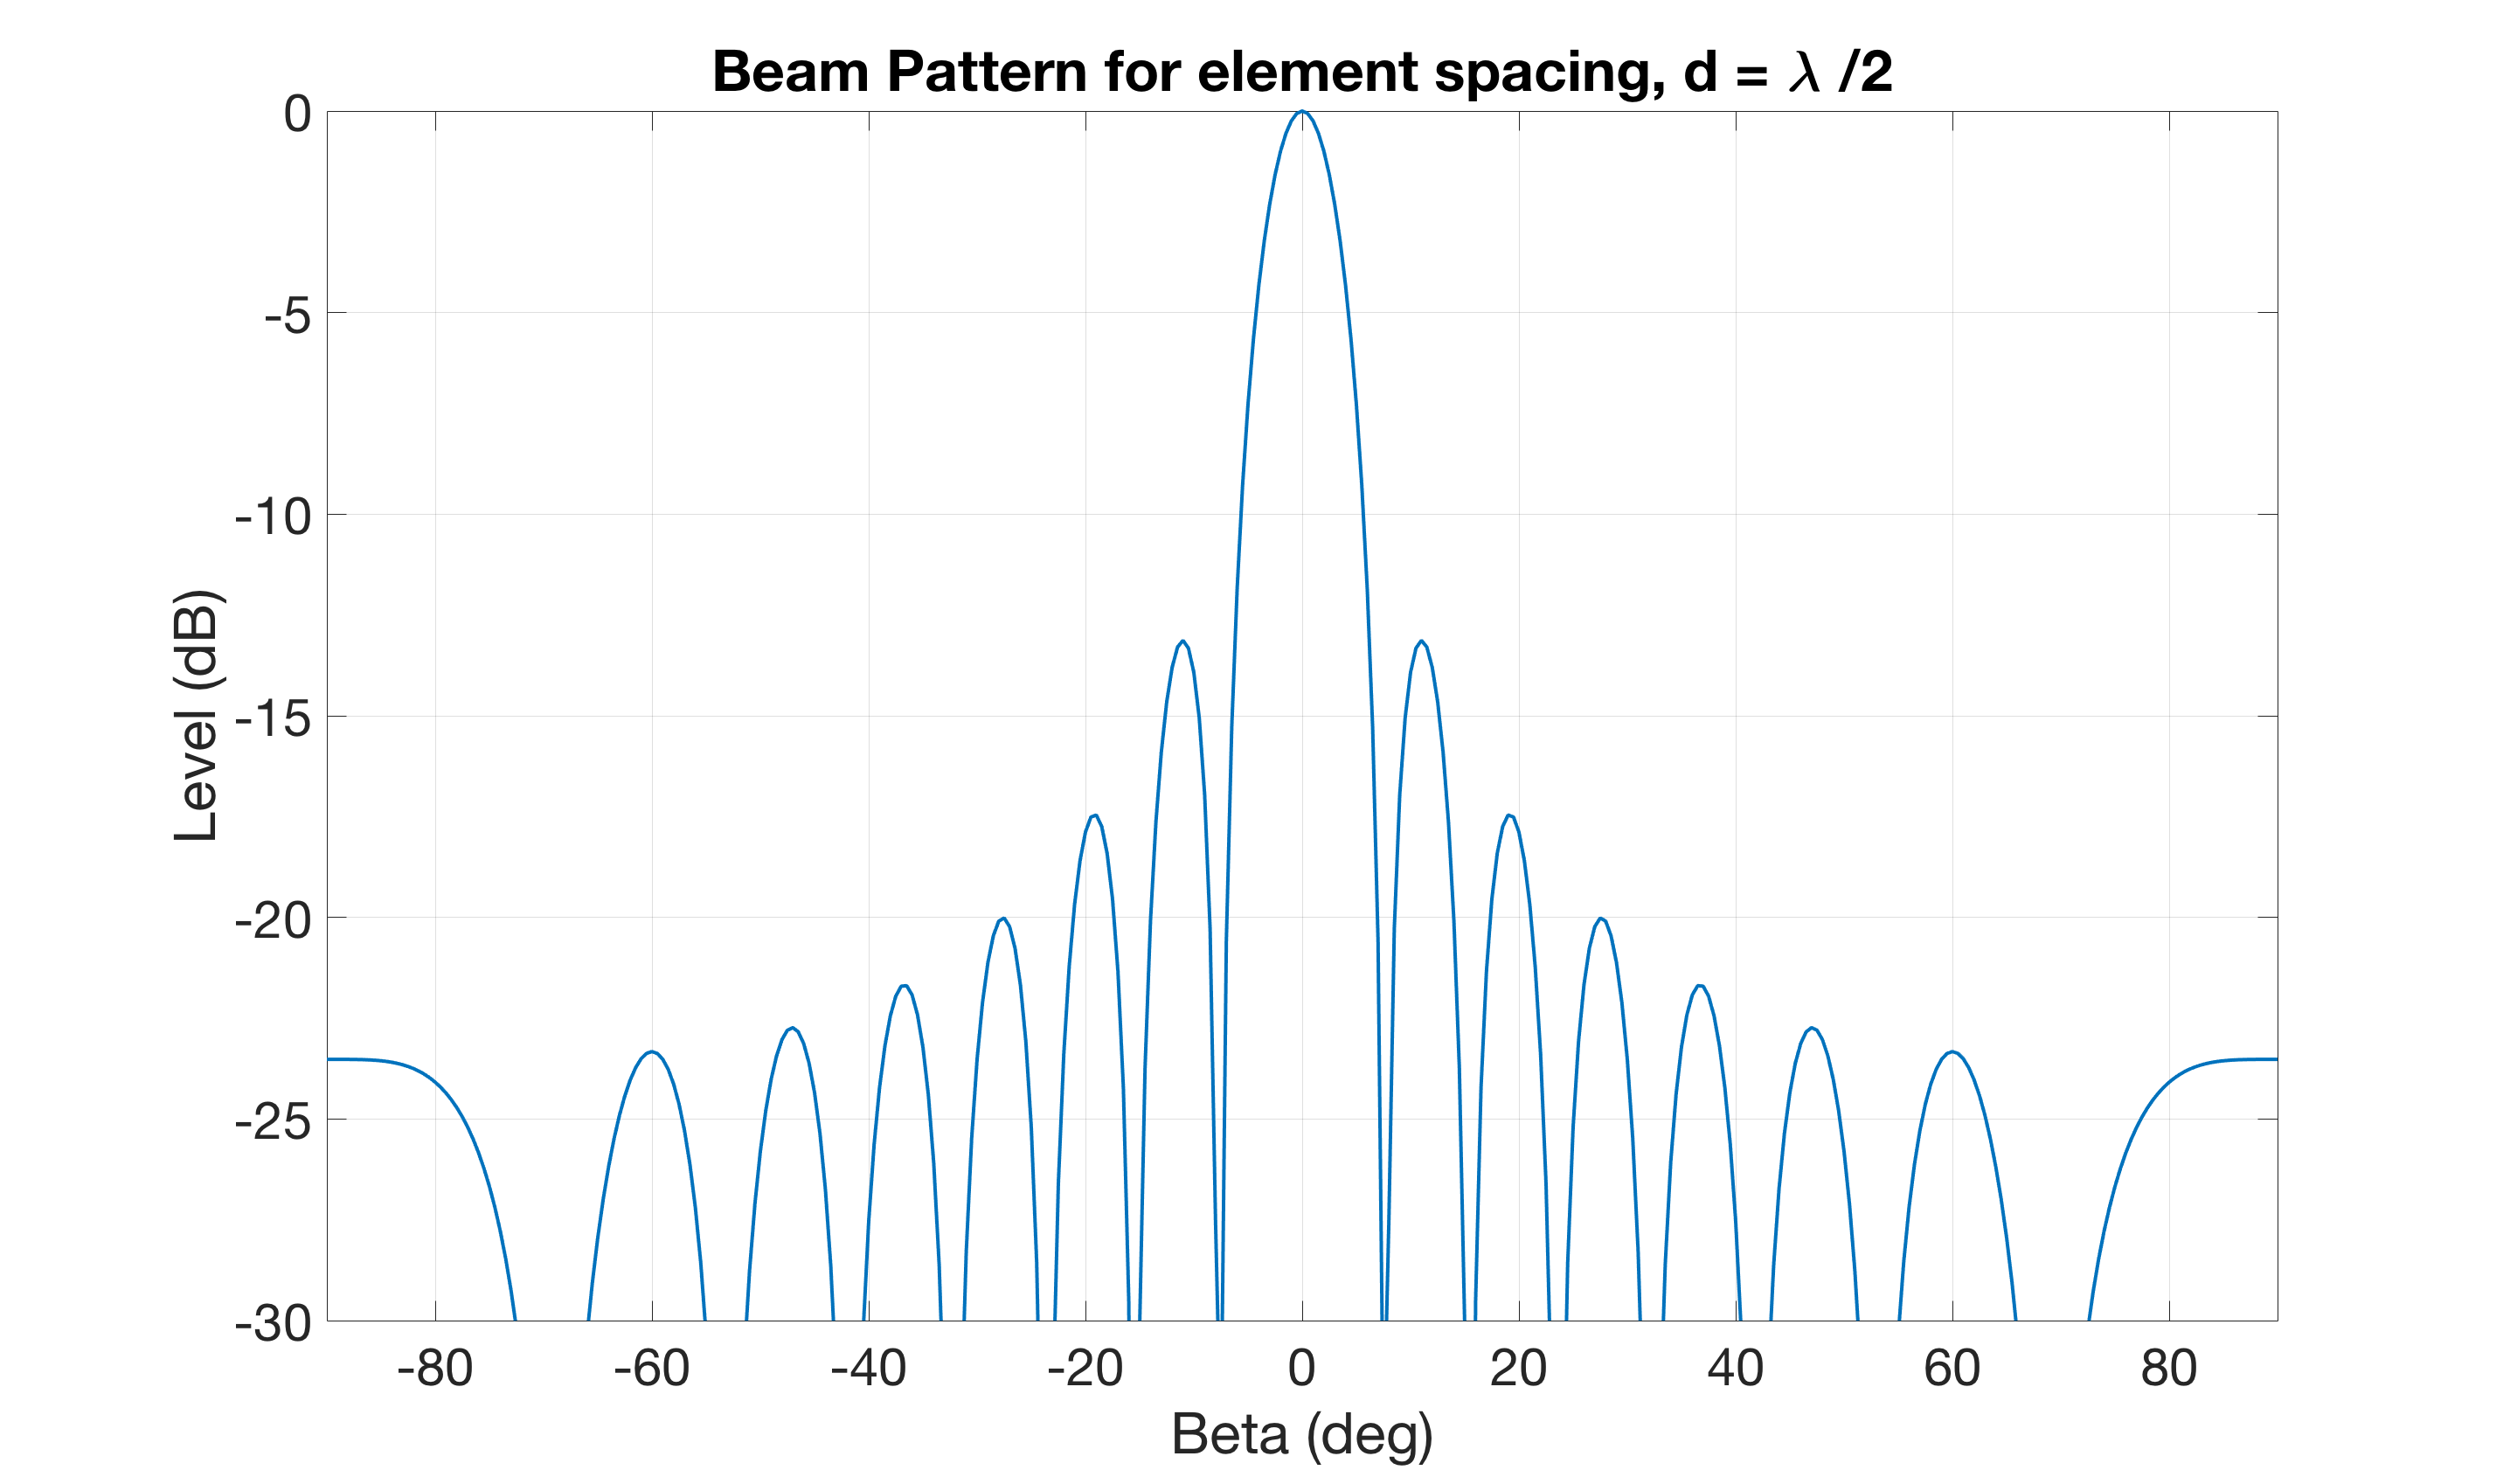
\includegraphics[width=95mm]{usp7_1.png}
}
\subfloat[Frequency, $\textit{f} = 100 Hz$]{
  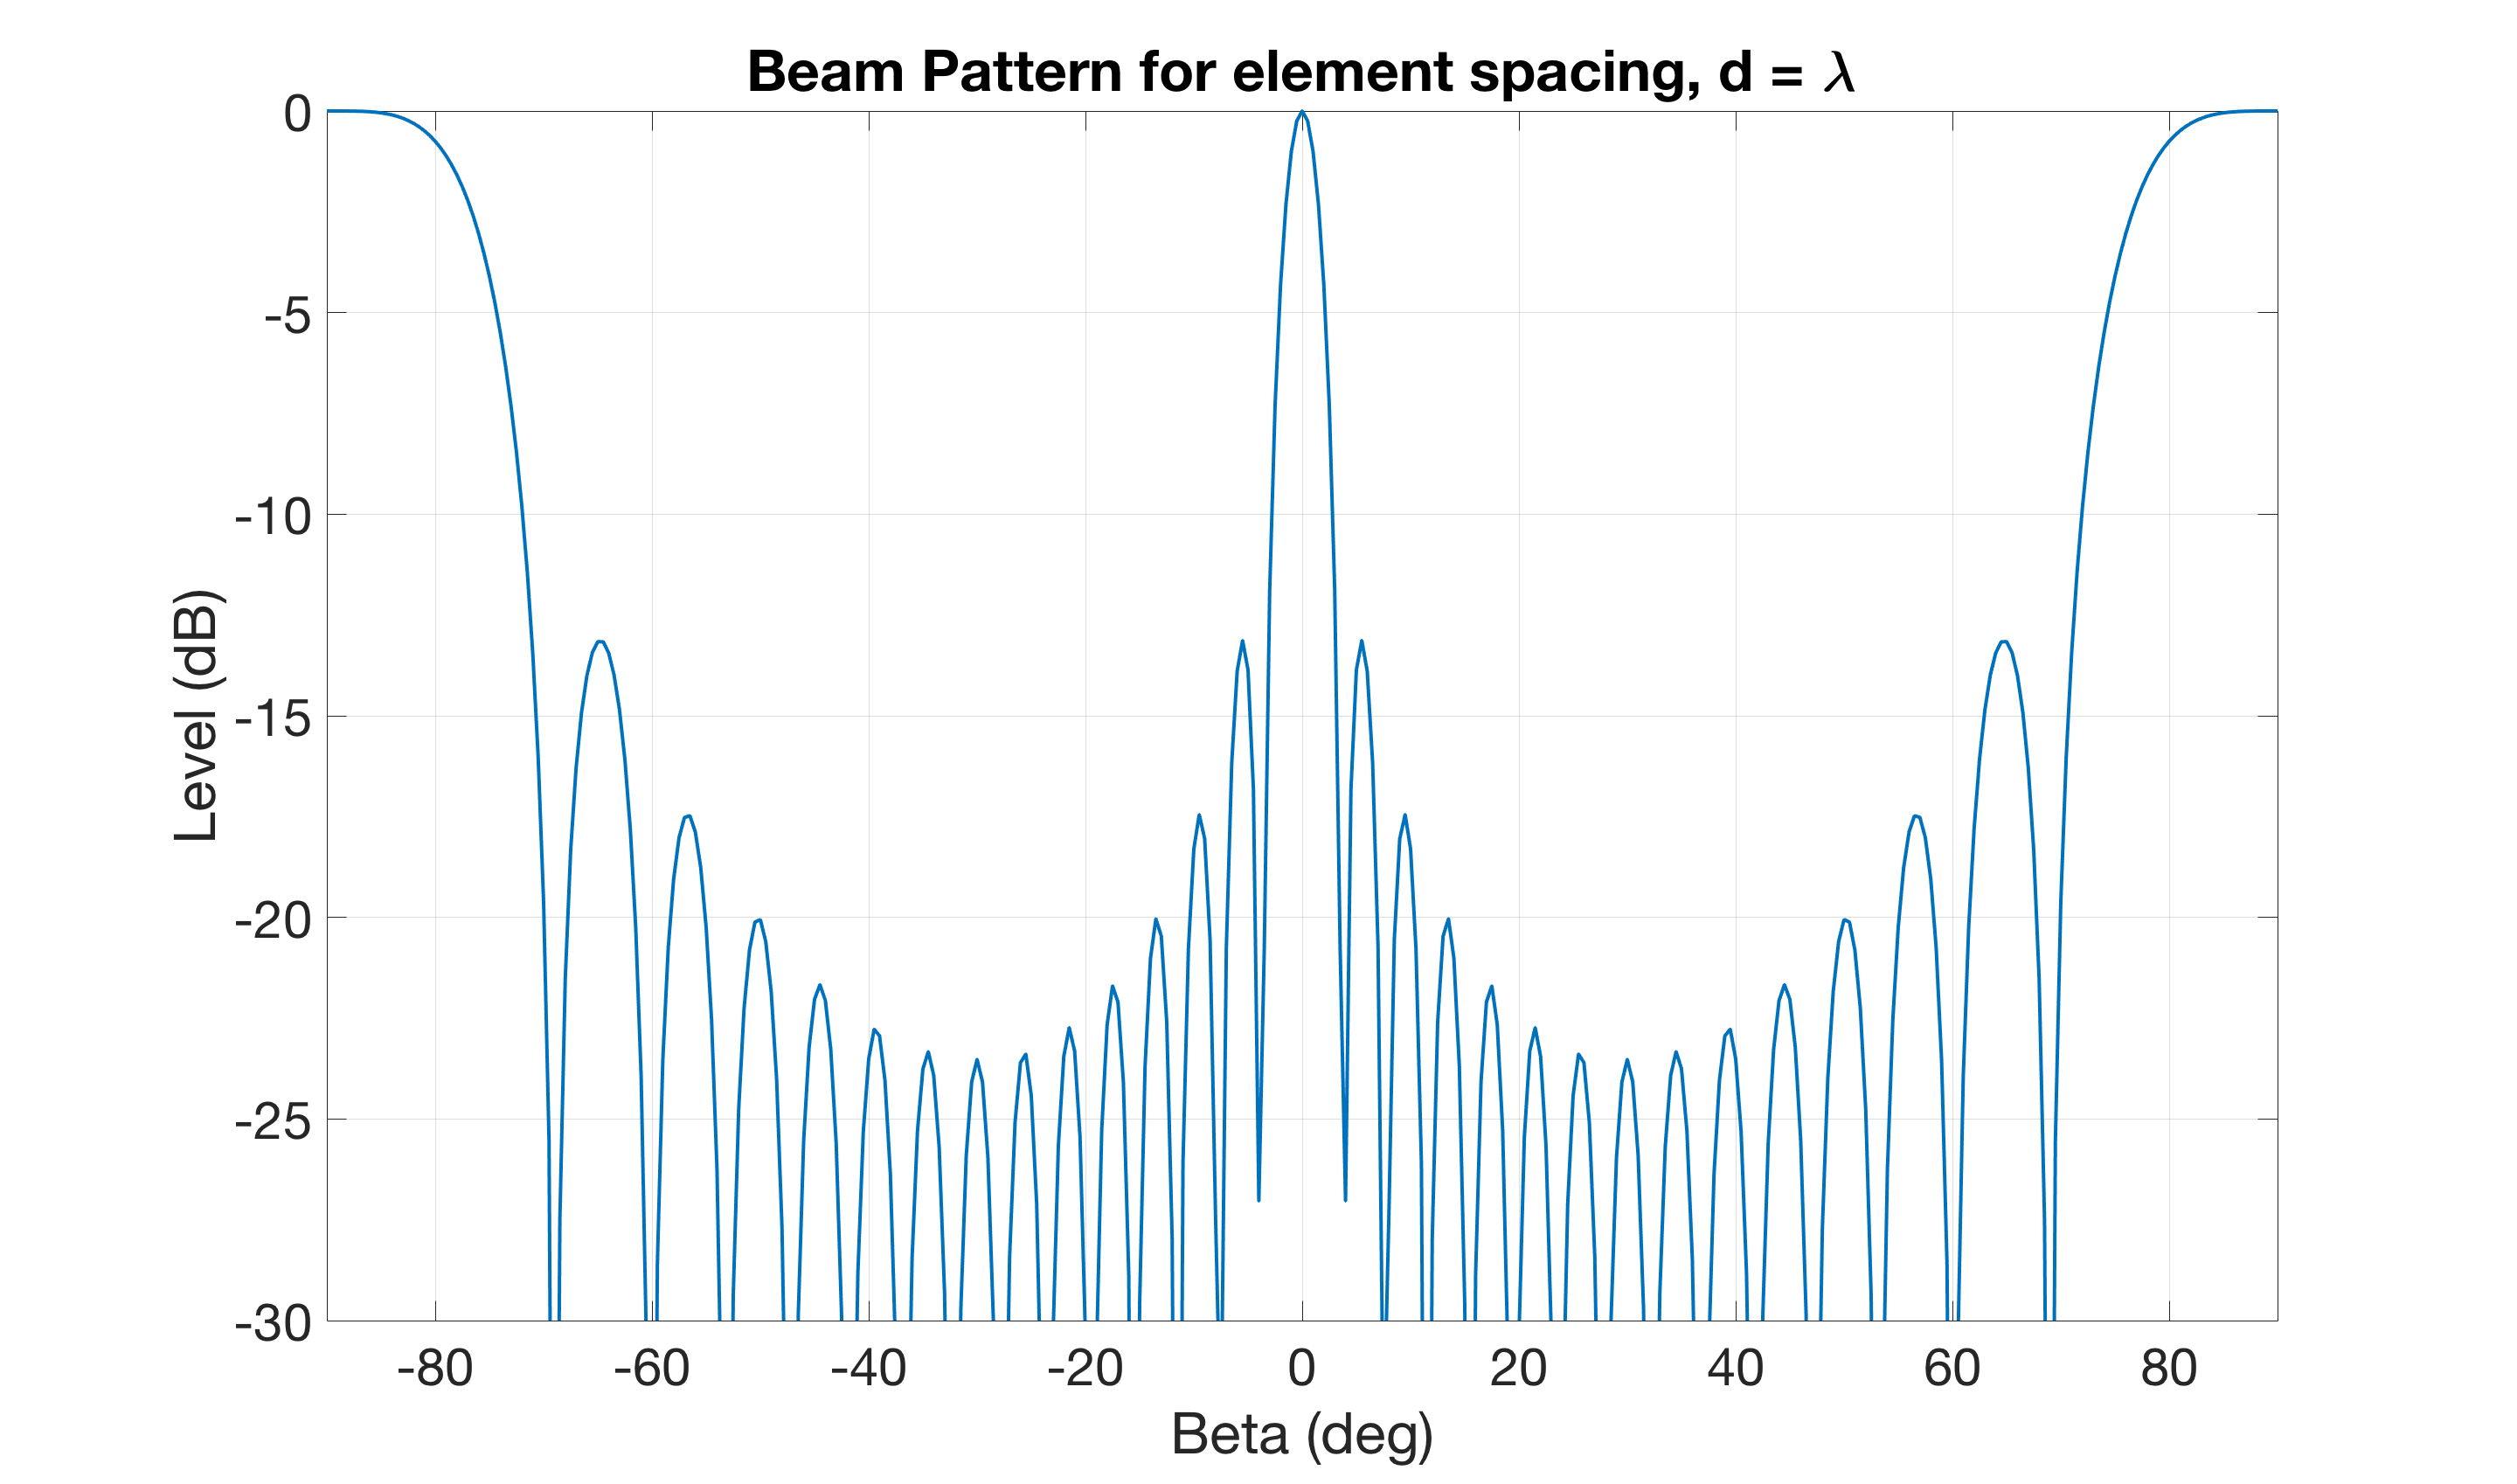
\includegraphics[width=95mm]{usp7_2.png}
}
\newline
\subfloat[Frequency, $\textit{f} = 1 kHz$]{
  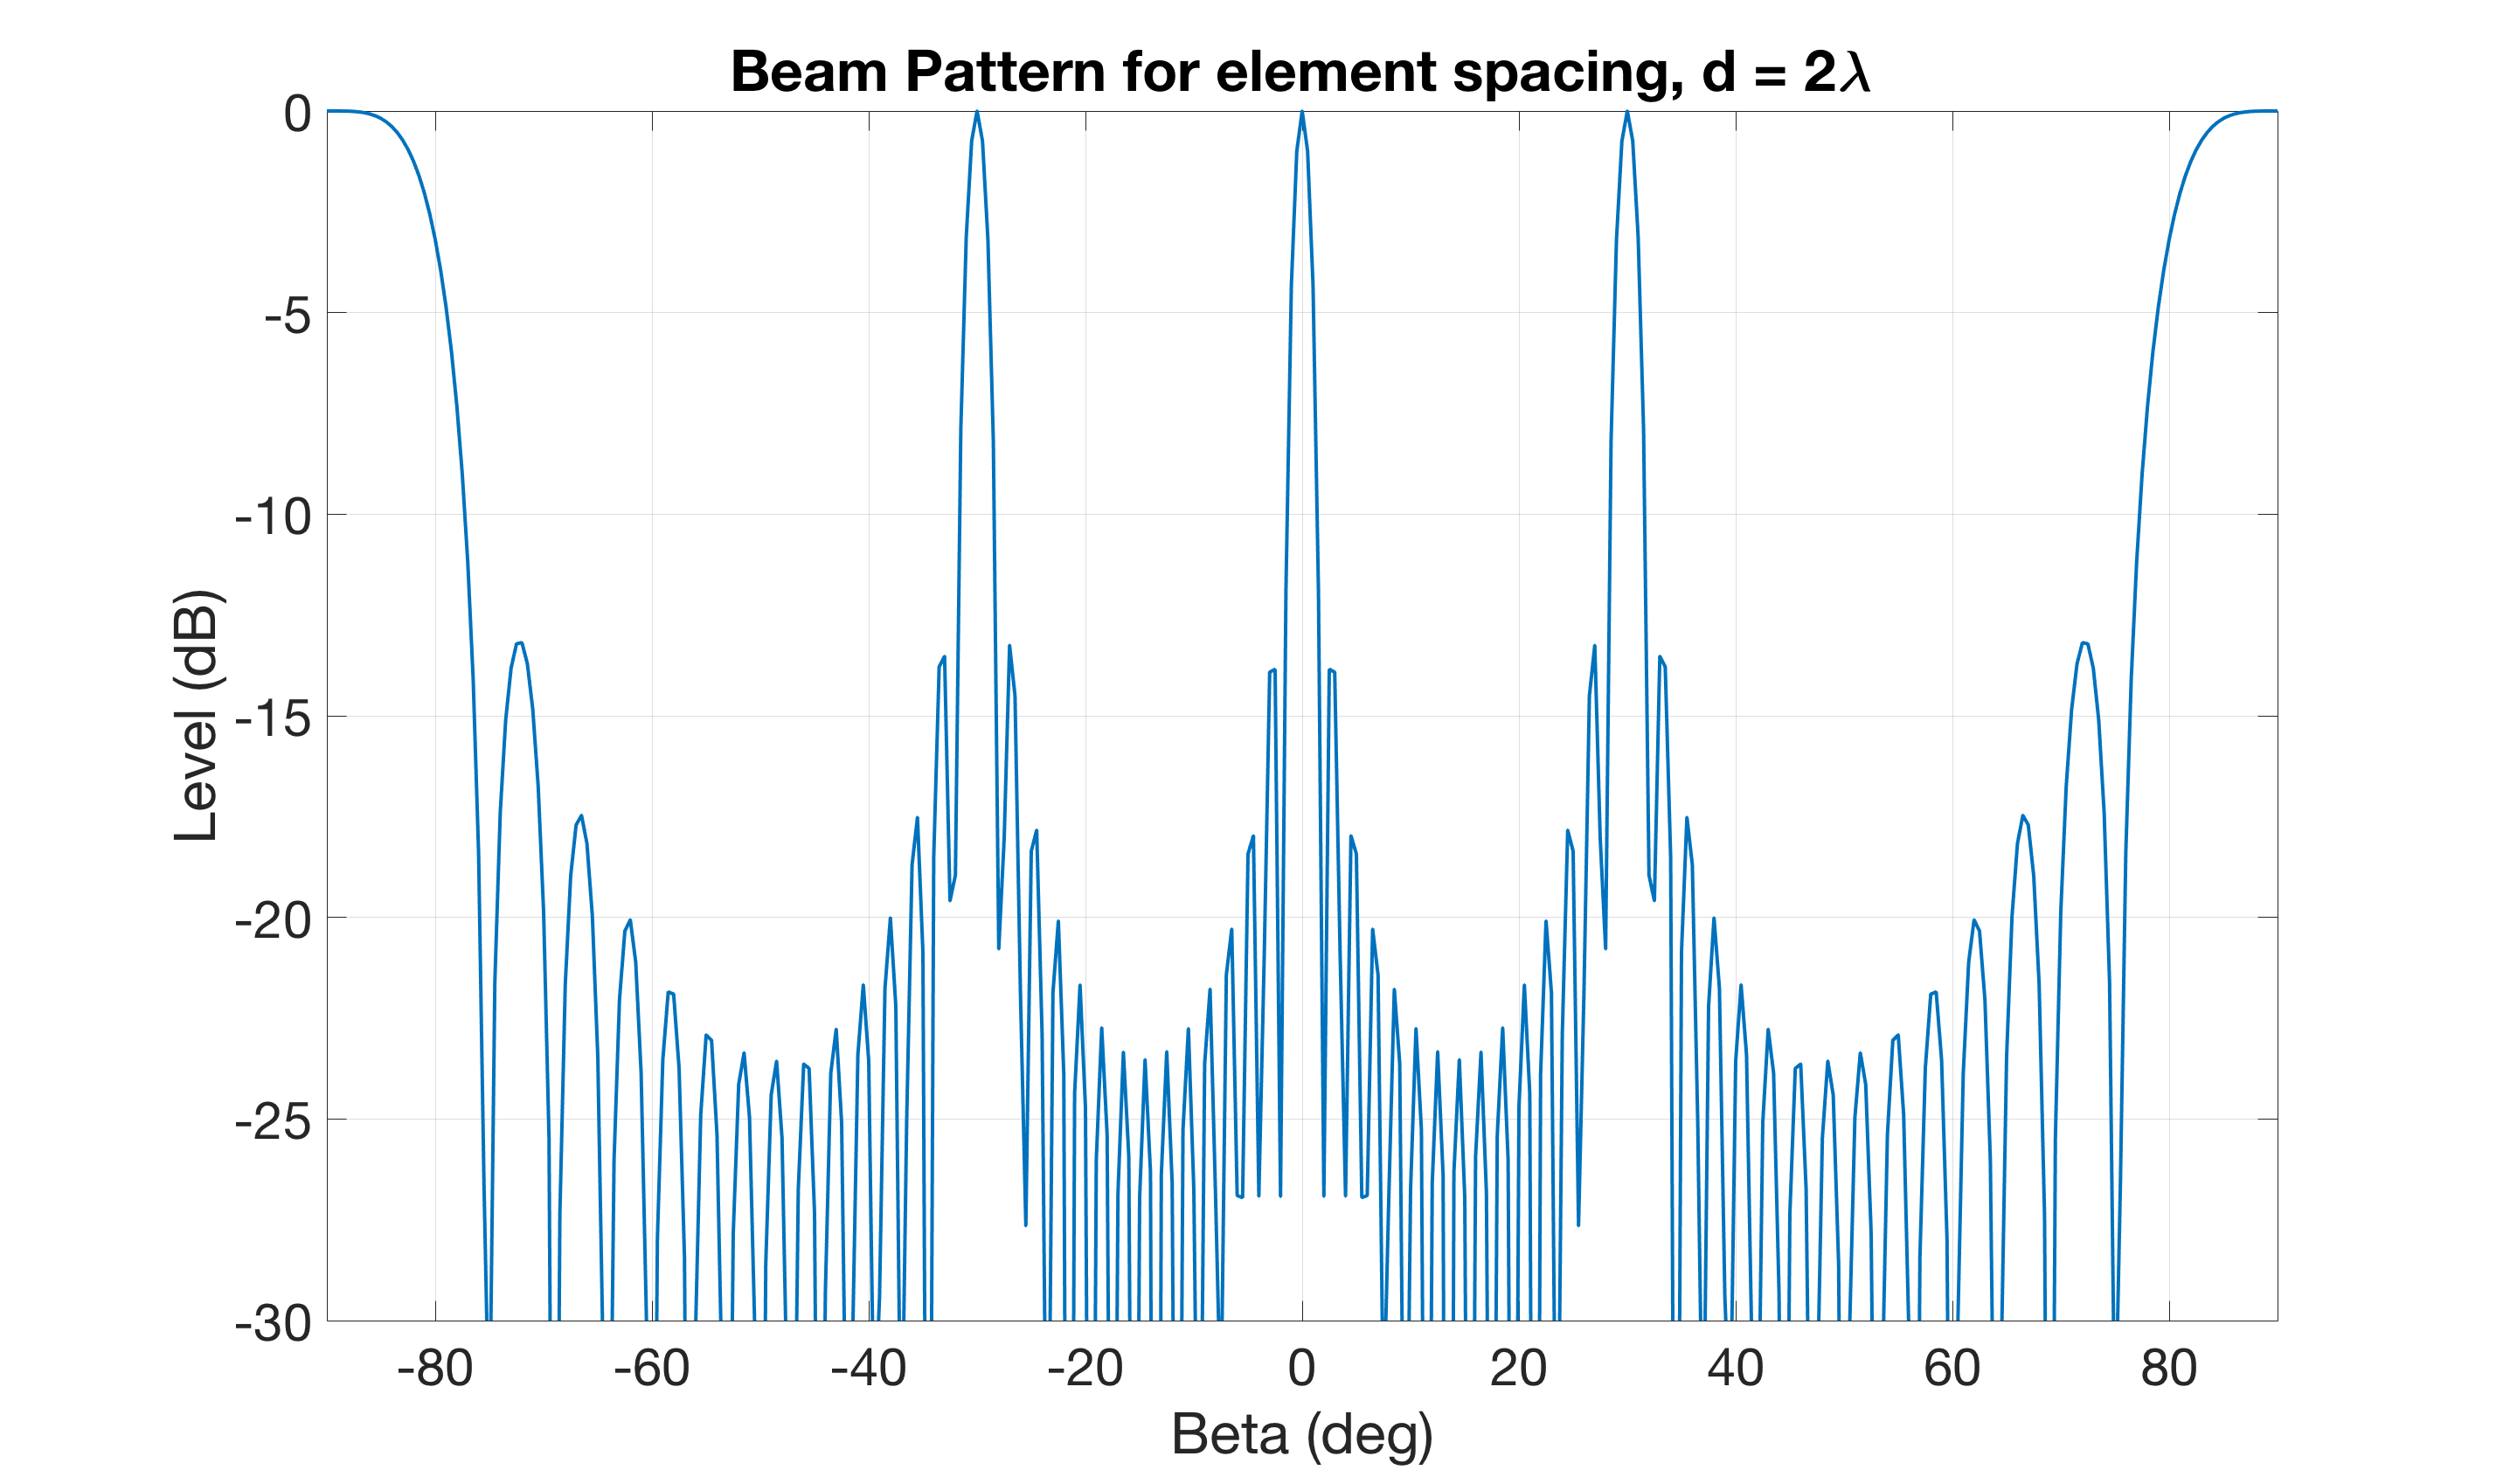
\includegraphics[width=95mm]{usp7_3.png}
}
\subfloat[Frequency, $\textit{f} = 10 kHz$]{
  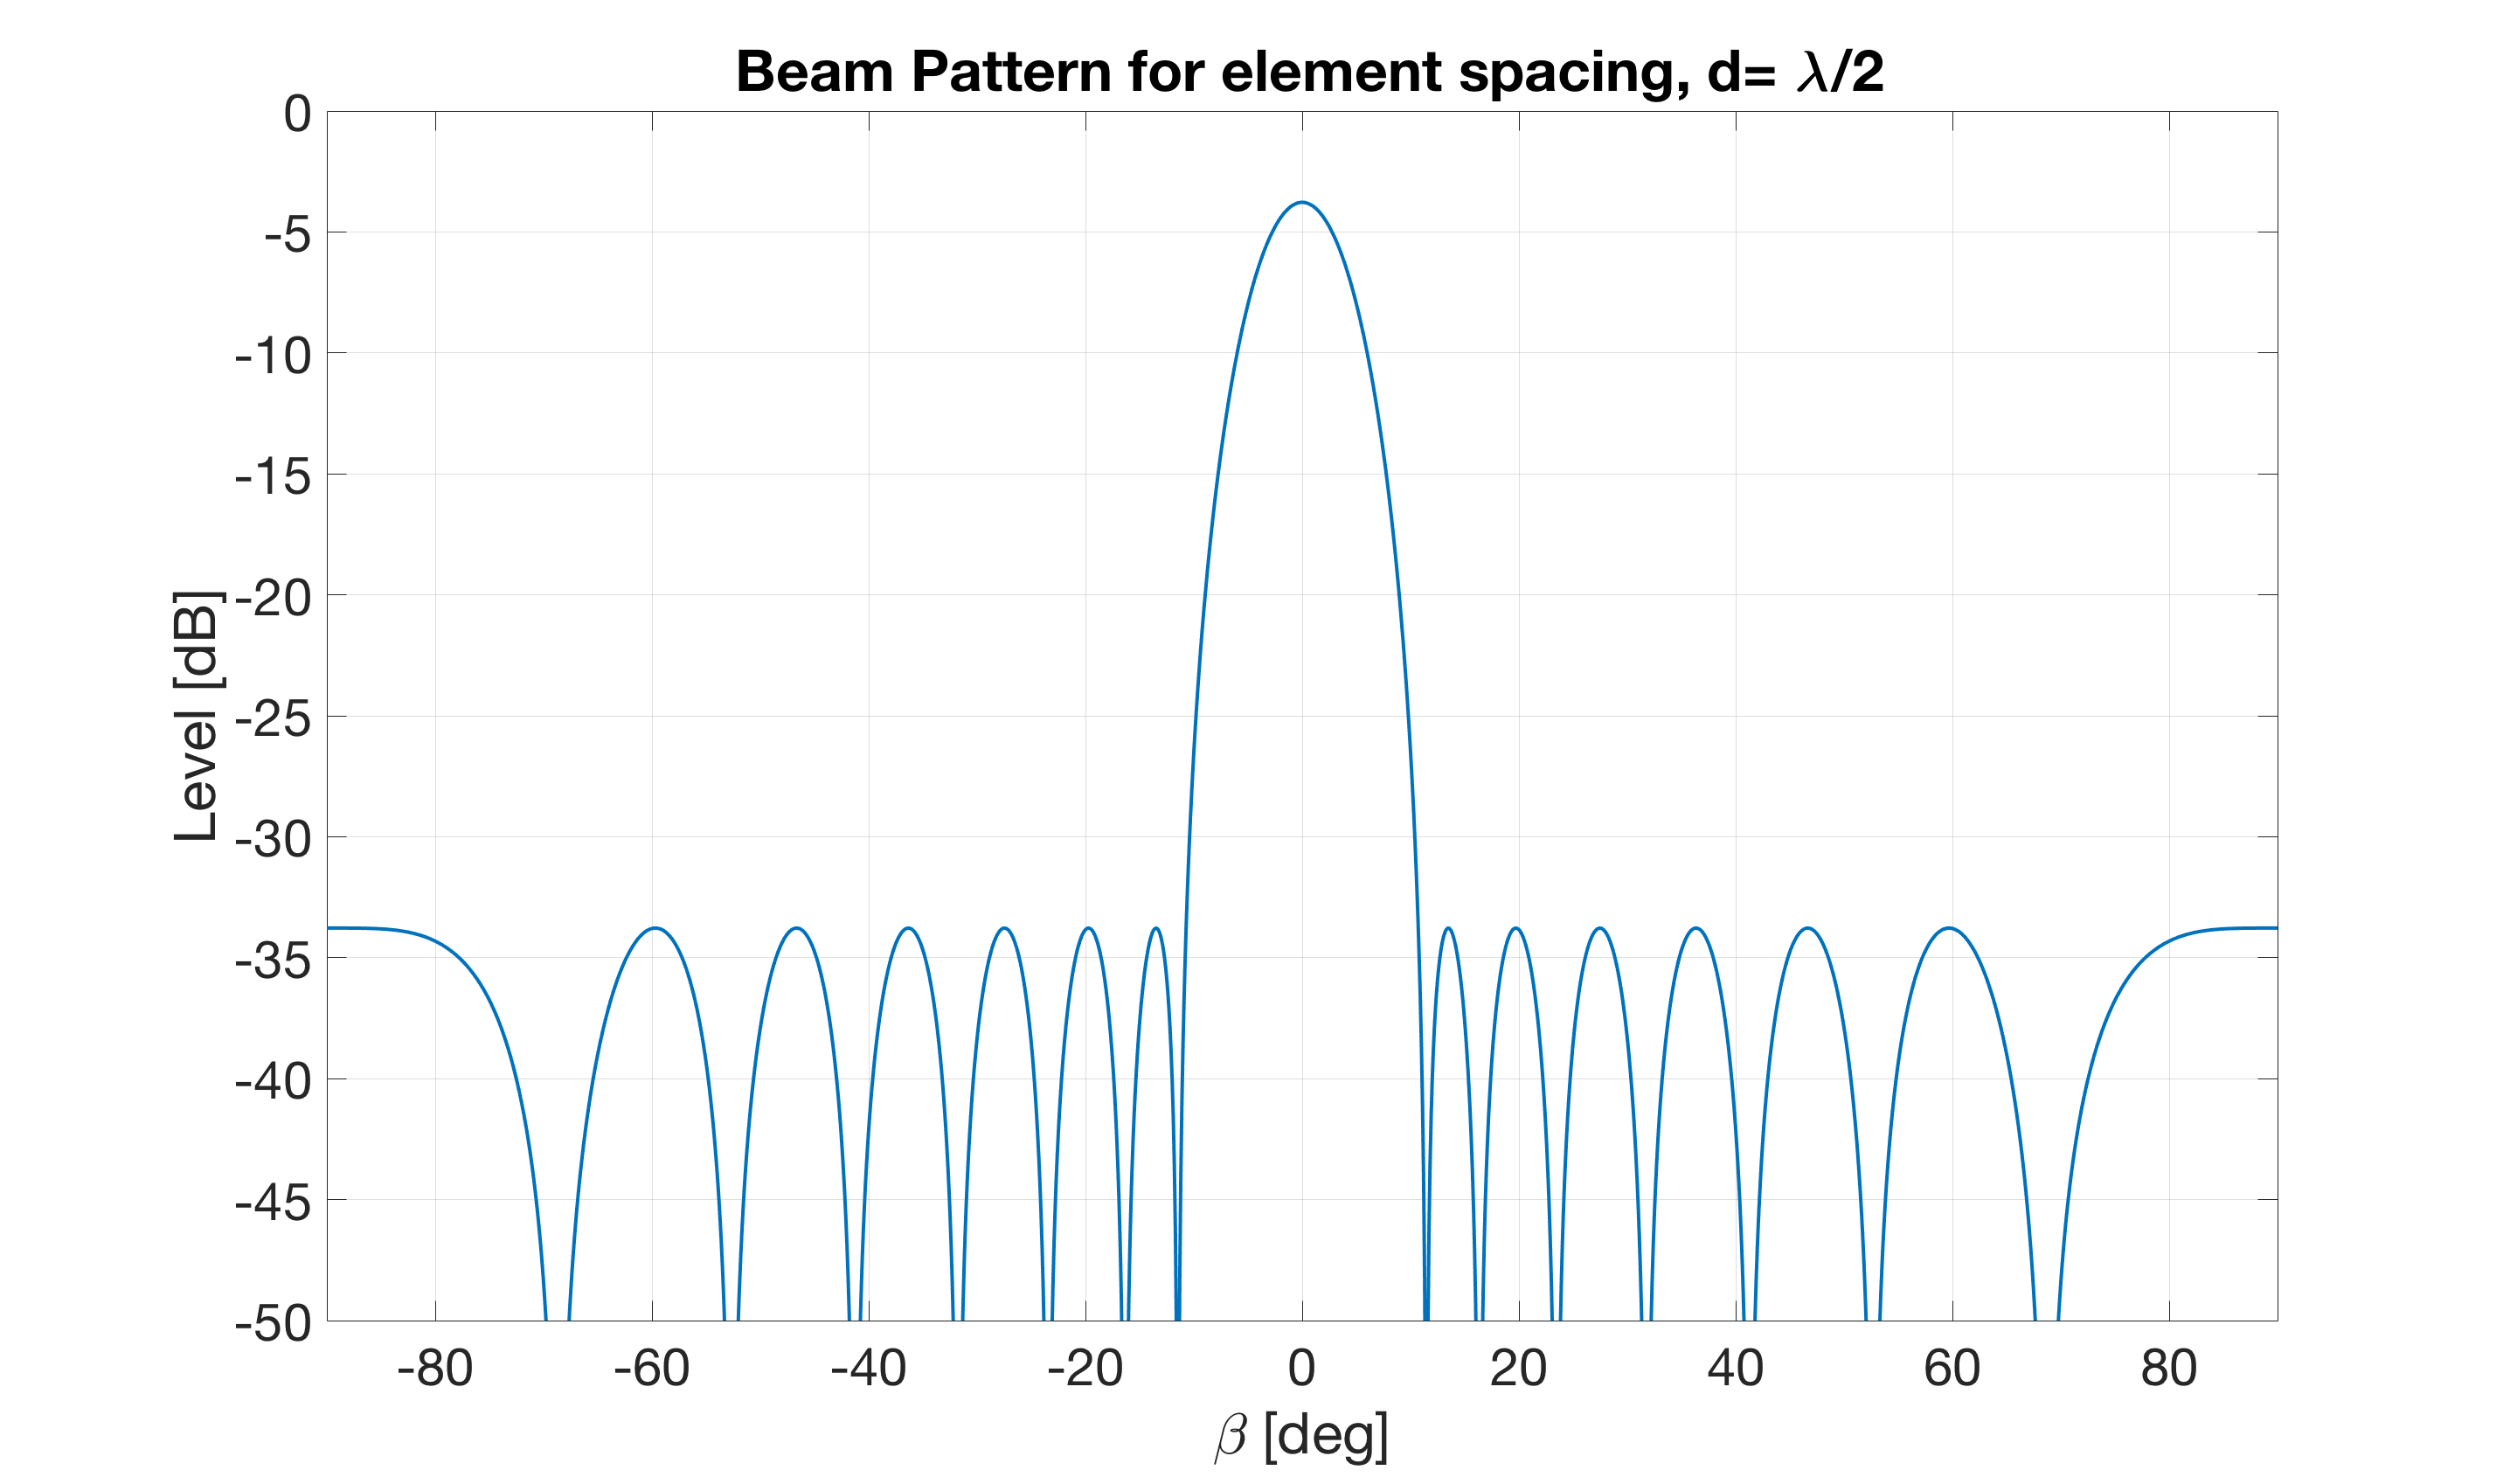
\includegraphics[width=95mm]{usp7_4.png}
}
\newline
\hbox to 18.5mm{}% !!
\subfloat[Frequency, $\textit{f} = 100 kHz$]{
  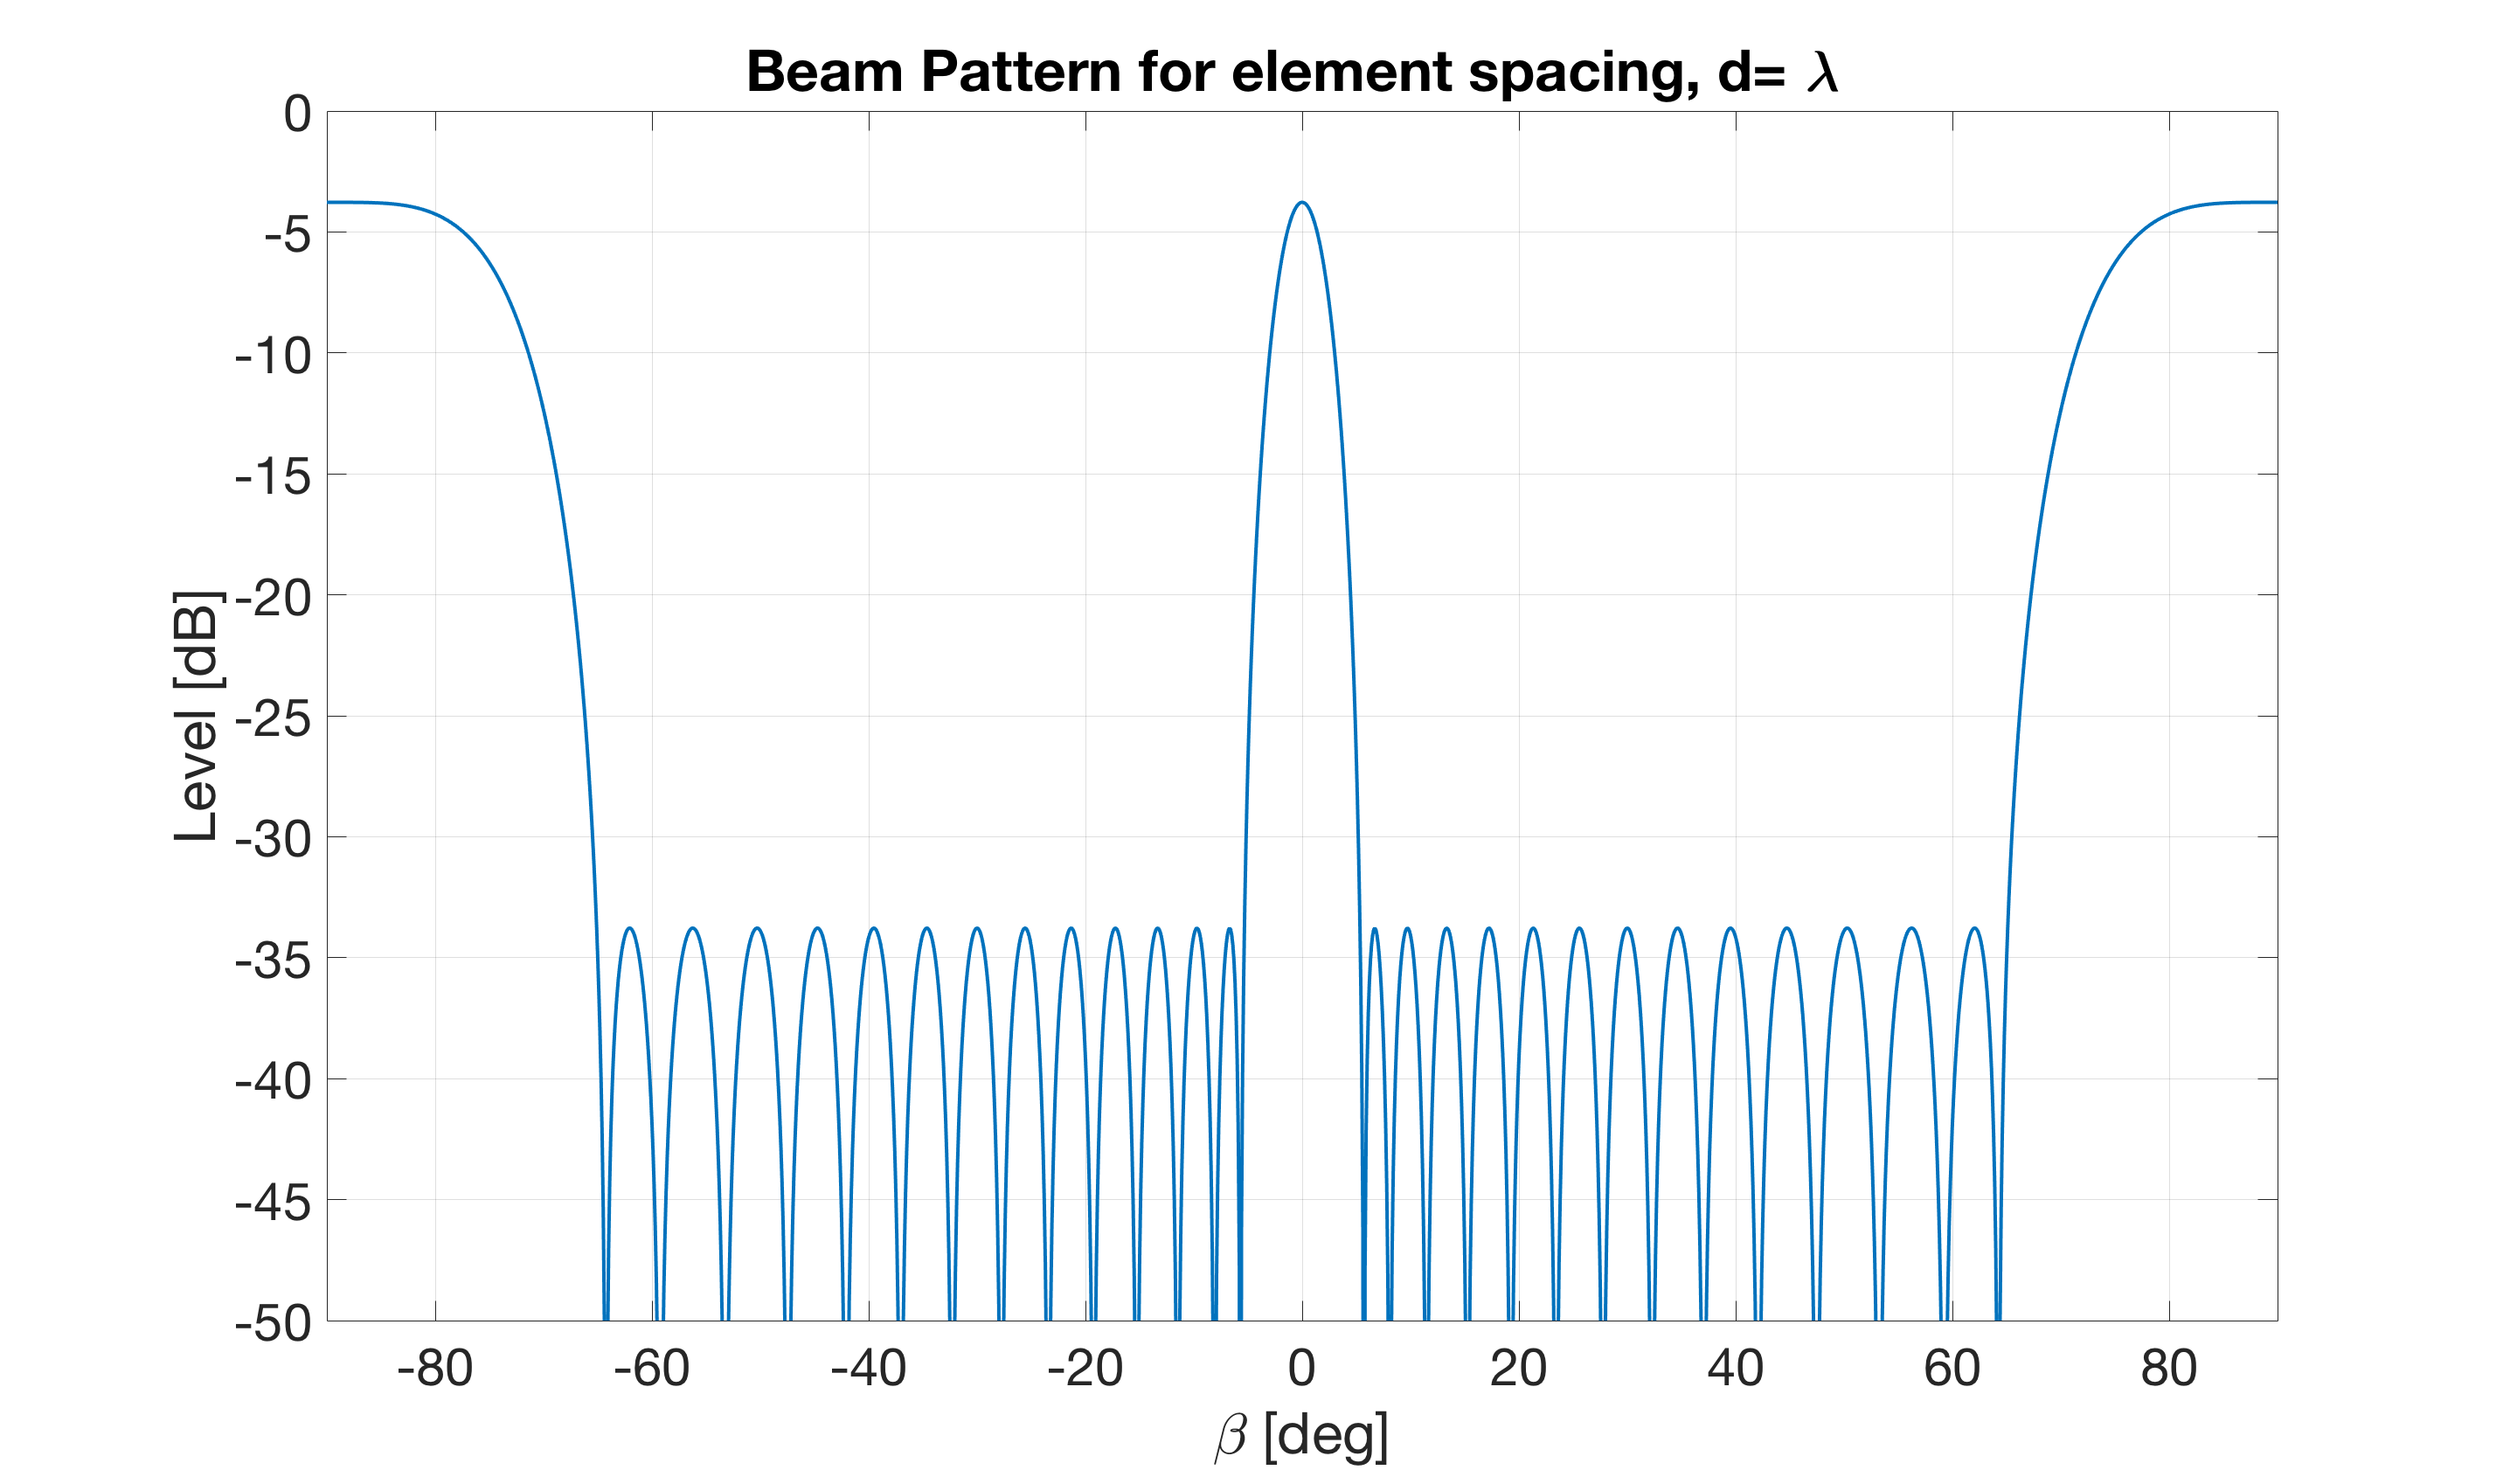
\includegraphics[width=90mm]{usp7_5.png}
}
\caption{ Pressure distribution observed at various frequencies }
\end{figure}
